\chapter{文字編輯器}
  很久以前我剛接觸電腦時,看到入門的人煞有其事的介紹editor,文字編輯器,我想這
  有什麼好講的,不就打打字後存檔嗎? 但是後來才發現代誌不是像憨人想得那樣而已。
  尤其對於是軟體開發者來說,editor是跟空氣一樣的,先來一些菜鳥觀念介紹
  \\\\
  基本電腦文件觀念
  \begin{itemize}
    \item 文件內容只暫存在記憶體buffer中。存檔時才會把buffer東西寫到硬碟去。
    \item 檔案真實面貌裏面有很多看不見的字元, tab, space, 換行LFCR等等,
      其中要小心的是換行字元,dos/windows是\verb=\x10\x13, unix下只有\x10=。
    \item 命令模式與編輯模式是標準傳統都會有的編輯器兩個模式,一個用來做命令,
      例如存檔,開檔,copy/paste,移動游標,一個是真正寫作。兩個模式間需要特
      殊按鍵切換,通常就是ESC。
  \end{itemize}
  程式師的編輯器
  \begin{itemize}
    \item indentation : 這是縮排對齊的一個單位。在傳統c中以tab鍵為單位。但很
      多程式語言就不一定,編輯器應該要有快速indentation的使用鍵。
    \item variable searching: 編輯器能對定義的變數做搜尋。
    \item syntax validation: 能對程式語言語法做顏色表現,也能偵測語法錯誤。
    \item IDE and outside command: 能夠使用外部工具做很多開發到測試流程的整合。
    \item setup and plugin: 有特殊變數與語法提供給使用者添加功能。
  \end{itemize}
  特殊鍵與unix習慣
  \begin{itemize}
    \item emacs / vi習慣,GNU有個readline
      library常被很多軟體使用,他提供的一些移動快速鍵,例如ctrl-e到行尾,ctrl-k
      殺掉整行等等常被很多軟體使用,同樣vi這個編輯器有很多使用鍵也有他的習慣,
      總之兩種快速鍵系統都有人用。
    \item / 搜尋鍵是vi使用的,在firefox或一些軟體中也會使用。
    \item regular express 代表鍵,unix 世界中,regular express 是一種用某種字元
      代表特殊意義的表示手法。例如\verb=^=表行首,\verb=$=表行尾。 這也常出現在
      一些軟體快速鍵中。
    \item Meta key 古早 Sun 鍵盤有個菱形方塊鍵,此為 Meta 鍵,PC 鍵盤中常以左Alt
      代表。 一些快速鍵以 Meta key 搭配其他鍵形成, 像\verb=M-F, M-%=。
  \end{itemize}
  上手前準備
  \begin{itemize}
    \item 英文打字一定要會,左右兩手手指放在asdf  jkl;上面控制a-zA-Z0-9。
    \item 免費英打遊戲可以去網路上找很多,要能盲打。
    \item 到最後,連中文輸入都盲打。
  \end{itemize}
  以上有些東西都是慢慢習慣的,一開始可能覺得很多,但最後就是習慣知道有哪些,
  這沒辦法快,只能慢慢才知道。

  \section{vim}
    本來在學校是用emacs的,後來到公司後,大家都用vi,還是傳統的vi,我很快就
    改用vi,到現在已經完全變vim了,vim的好處就是兩隻手永遠都在asdfjkl;上面。
    \begin{verbatim}
一。從命令到編輯模式
a	:將游標放到目前游標後一個字元,開始文字編輯模式。append
i	:將游標放在目前游標位置,開始文字編輯模式。insert
o	:將游標放到下一行起始位置,開始文字編輯模式。open new line
比較常用就是i,a,o,I,A,O了,將來多試幾次就好了,就很熟悉了。

二從編輯到命令
ESC	:沒事多按逃脫鍵,有益身體健康。

三命令模式中的其他命令
在命令模式中的按鍵就很多了,這些需要好好熟練一下了。
在vi命令模式裡面,有的按鍵按完後他還是在命令模式,有的改個字元或copy/paste後
又回到命令模式,有的就一去不回頭變成文字編輯模式了。
有些按鍵會把你原本想改的內容做特殊的定位,例如要改個word,也會把你帶離命令模式

檔案
:q		離開vi
:e xxxx		編輯xxxx
:w		存檔
:w xxxx		另存檔案xxxx
:q!		不存檔強迫離開
:w!		強迫存檔
:wq		存檔與離開

游標移動
h,j,k,l		往左,往下,往上,往右
0		到行首
$		到行尾
^		到這行的第一個非空白字元

w,W		到下個字, 到下個非空白的字
b,B		回上個字, 到上個非空白的字
e,E		到這個字的字尾, 到下個非空白的字字尾

Ctrl-F ,Ctrl-B	往後一頁,往前一頁
gg              表示檔頭
G		到檔尾
:n		到第n行 (所以到檔頭就是:1)
Ctrl-G		顯示第幾行
J		合併兩行

搜尋與取代
/
/pattern        尋找pattern
?pattern        往上尋找pattern
n               再往下尋找
N               再往上尋找
*               目前游標下的字串尋找
#               跟 * 一樣,只是往上找
:s/pattern/str/cgi
                搜尋pattern取代str
                其中:跟s間是指定範圍(range),沒設就是游標這行 
                1,10 表示 1-10行
                %    表示整篇
                最後cgi
                c 表示confirm尋問
                g 表示global全部
                i 表示ignore不分大小寫

常用字元字串處理
cc              改變整行
dd              砍掉整行
yy              拷貝整行(yank whole line)
p,P             貼上(paste)你最近砍掉或拷貝的

cw              改變一個字
d$              砍到行尾
ye              拷貝到這個字尾

r,R             取代一個字元, 取代整行
u,U             undo 最後修改,UNCHANGE整行
x,X             砍一個字元, 往回砍個字元(等於按backspace)

重複的處理
.               重複剛剛的命令或輸入

indentation
>>              往右一個indent
<<              往左一個indent
=               這行indentation
15==            15行indentation
gg=G            表示檔頭到檔尾做一次indent

大小寫變換
~               大小寫互換
3~              三個字元變換大小寫
VIM的大小寫變換
guw             整個字小寫
gUw             整個字大寫

這些試試看
ce, 3x, 5dd, 10w, d0, y$, 5G
	  
vim的多檔與多窗
:set hidden     這設定buffer被改動後,能夠先不儲存而換到別的buffer去
:e xxx          編輯xxx
:buffers        列出所有編輯檔
:bn             n是數 b1 b2 b3....表是開第n個buffer
:bdn            n是數:bd1 :bd2 表示殺掉第n個buffer 

:new            一個水平新窗
:vnew           開個垂直新窗
:only           只留一個窗窗

C-w j k h l     移到下 上 左 右 窗去
C-w w           到下個視窗
C-w c           關掉窗子
\end{verbatim}
    \subsection{vim小技巧}
      以上基本使用,熟悉一個下午就可以,除了基本使用外,有些使用如下
      \subsubsection{syntax color}
      \begin{verbatim}
:syntax on
      \end{verbatim}
      設定程式語言語法顏色,不過我剛開始工作時,資深工程師連這個都不用的。
      非常傳統的unix/vi。他們腦袋真的非常仔細,不需要花俏的東西。

      \subsubsection{顯示行號}
      \begin{verbatim}
:set number
      \end{verbatim}
      在遠距開會除錯時用來跟同事溝通

      \subsubsection{fold}
      程式常是小單位組成,最常見的就是一個 block ,由大括號 \{ \},包住,
      fold 是合併 block 內容成一行,讓整個檔案看起來是大塊邏輯組成即可。
      但有時自動幫我們做這些也很煩,要開開關關
      \begin{verbatim}
za    toggle 開變關,關變開
zo    open
zc    close
zA    這三個跟上面三個一樣,只是作用在檔案全部
zO
zC
      \end{verbatim}
      fold 方法有 manual, indent, syntax
      \begin{verbatim}
:set foldmethod=indent
:set foldnestmax=10
:set nofoldenable
:set foldlevel=2
      \end{verbatim}
      \subsubsection{tag symbol searching}
      用ctags命令對一堆c sources產生tag 檔,就可以跳來跳去想看的變數 symbol。
      \begin{verbatim}
      $ ctags -d -t -w `find . -name "*.[ch]"`
      $ find . -name "*.[ch]" | xargs ctags -a -d -t -w
      或者
      find . -name "*.[ch]" > files
      find /usr/include >> files
      ctags -L files
      \end{verbatim}
      -d 表示 \verb=#=define的macro, -t 表示typedef的也放進tags,
      -w 表示不要warning.
      \\\\
      幾個重要命令:
      \begin{itemize}
        \item ta myvar 跳到myvar這個tag
        \item ts myvar 列出有所有myvar tag的檔案。
        \item pop 跳回去原來地方。
      \end{itemize}
      幾個重要快速鍵:
      \begin{itemize}
        \item ctrl-] 跳到游標指的symbol,
        \item ctrl-T 跳回去原來地方。
        \item g ctrl-] 列出所有的symbol的檔案讓你選
        \item \% 跳到相對應的 block 起始或結尾,通常我們 function, for, if
          起始結尾都是 \verb={ }= 所以用 \% 可以跳到相對應的這兩個地方。
      \end{itemize}
      還有
      \begin{itemize}
        \item gd 表示尋找目前游標下字串的原始local變數
        \item gD 大寫D表示全域變數尋找
      \end{itemize}

      \subsubsection{external command}
      例如使用:!ls來使用ls命令。使用:make 來做 make 。當用 make 時,cn
      與 cl 是列出錯誤訊息並跳到發生錯誤行的命令。

      \subsubsection{autocomplete}
      ctrl-n 可以 autocomplete, autofill 自動補全打一半的字,不過這只是根據
      現有檔案內有的字串,要像一般 IDE 那樣,必須裝特別 vim plugin 才行。

      \subsubsection{vimdiff}
        同時編輯兩個檔案並用顏色標出兩者不同處,這通常是用來解
        branch merge後conflicts時所用。使用\verb=[c ]c=跳到下一個兩邊不一樣
        的地方。解完後,顏色不同的地方會自動消失,我跟同事使用時,同事非常
        驚豔,想說怎麼這麼好用,完全是他們不會用而已。
      \subsubsection{.vimrc}
      vim有豐富的內部變數設定,也有條件式的script可以使用與設定變數,像之前
      的syntax on這個就是命令之一,只是冒號: 都不用打了。所以可以把這些設定
      寫到\$HOME/.vimrc去,則整個起來的環境就是個人使用環境。
      \\\\
      一個簡單的.vimrc
      \begin{verbatim}
if has('syntax') && (&t_Co > 2)
	syntax on
endif

set autoindent
set title
set ruler
set hidden
set fileencodings=utf-8,big5
set fileencoding=utf-8
set encoding=utf-8
function Setsts()
  if &sts == 0
    set sts=2 sw=2
    set expandtab
  elseif &sts == 2
    set sts=4 sw=4
    set expandtab
  elseif &sts == 4
    set sts& sw&
    set noexpandtab
  endif
endfunction
map <F2> :call Setsts()<BAR>set sts?<CR>
map <F3> :set paste!<BAR>set paste?<CR>
map <F4> :set hls!<BAR>set hls?<CR>
map <F5> :bp<CR>
map <F6> :bn<CR>
map <F7> g^]
map <F8> ^T

if has("autocmd")
  filetype plugin indent on

  autocmd FileType text set sts=2 sw=2 expandtab textwidth=78
  autocmd FileType sh set sts=4 sw=4 expandtab
  autocmd FileType perl set sts=4 sw=4 expandtab
  autocmd FileType python set sts=4 sw=4 expandtab
  autocmd FileType php set sts=4 sw=4 expandtab
  autocmd FileType spec set sts=4 sw=4 expandtab
  autocmd FileType c set sts=4 sw=4 expandtab cindent
  autocmd FileType javascript set sts=2 sw=2 expandtab
  autocmd FileType vim set sts=2 sw=2 expandtab
  autocmd FileType rst set sts=2 sw=2 expandtab
  autocmd FileType tex set sts=2 sw=2 expandtab
  autocmd FileType sgml set sts=2 sw=2 expandtab
  autocmd FileType html set sts=2 sw=2 expandtab
  autocmd FileType conf set sts=2 sw=2 expandtab
  autocmd FileType yang set sts=2 sw=2 expandtab autoindent

  autocmd BufReadPost *
    \ if line("'\"") > 0 && line("'\"") <= line("$") |
    \   exe "normal g`\"" |
    \ endif

endif " has("autocmd")
      \end{verbatim}
      其中那些set就是設定變數值,沒有等號的就是設true。sts是softtabstop表示按
      tab時是跑幾格,sw是shiftwidth,表示使用\verb=>> <<= 時,indent時,是跳幾格。
      expandtab是說如果有8個space時,要不要把他自動變成一個tab表示。
      而其中很有用的就是map這個設定快速鍵使用。這個必須:help map就可以看到文件
      。通常搜尋vim網站,可以看到很多人寫的小設定了,可以直接拿來使用就好。
      \\\\
      其中F7與F8用上了特殊鍵ctrl,但\verb=^] ^T=兩個值是不能用打字ascii方式輸入
      ,而必須真的是這兩個鍵的binary值,所以必須ctrl-v ctrl-]輸入\verb=^]=,
      ctrl-v ctrl-T輸入\verb=^T=。

  \section{emacs}
    emacs的就稍微放一下以前寫的命令小抄,我已經完全忘光不用emacs了。不過資深白人
    同事,使用 emacs 都嚇嚇叫,出神入化
    \begin{verbatim}
檔案
C-x C-c		:離開 emacs
C-x C-f		:開檔
C-x C-s		:存檔
C-x C-w		:另存新檔

游標移動:
C-a		:移到行首
C-e		:移到行尾
M-f		:向後移一個字
M-b		:向前移一個字
HOME		:移到檔頭
END		:移到檔尾
M-m		:移到這行第一個字元

常用的鍵
M-x		:執行一個emacs命令
C-g		:離開一個emacs命令
C-_		:UNDO
C-s		:搜尋  一直按一直往下找
C-r             :往上搜尋
M-%		:搜尋與替代(按!全部換掉,要不,會一個一個問按y/n回答)
M-C-s		:regular express 搜尋

M-DEL		:往前砍個字
M-d		:往後砍個字
C-k		:砍掉游標後所有字
M-t		:轉換兩字
C-x C-t		:轉換兩行
    \end{verbatim}
    一般說來在X 視窗下,我們可以用滑鼠就可以標示文字了,現在通常有兩個 buffer,
    一個是Window Manager 像 gnome, kde 提供的 clip board buffer, ctrl-c,
    ctrl-v,另一個是原本 X 提供的, 只要用滑鼠左鍵標好,可以按 shift 鍵調整,然
    後用滑鼠中鍵就可以paste了。 這如果按著 shift 鍵跟滑鼠左鍵可以更精確控制。
    emacs的區塊沒有所謂的column mode的區塊。
    \\\\
    區塊的標記:
    \begin{verbatim}
C-SPCE = C-@	:開始區塊標示,然後移動游標
		:如果想看到反白請先下emacs 命令"transient-mark-mode"
		:但如果用了這個,滑鼠的左鍵標示就看不到反白了喔。
C-x h		:標示整個編輯區(就是整個檔案)
C-w		:砍掉標示的區塊(用滑鼠右鍵按兩下或按del - 這個要20版以上的才有)
C-y		:把剛剛砍掉的或在區塊中的文字回存(也可以用滑鼠中鍵)

多檔與多窗
C-x 5 2		:開一個新窗子在新的frame
C-x 3		:開新垂直窗子在同一個frame
C-x 1		:只留一個窗子
C-x o		:改到其他(other)窗子
C-x b		:改到其他buffer(編輯區)
C-x k		:kill掉目前編輯區
C-x C-b		:列出所有編輯檔案

基本巨集
C-x (		:開始紀錄你所按的鍵
C-x )		:結束你所紀錄的鍵
C-x e		:執行剛剛紀錄的所有組合按鍵
M-n C-x e	:執行n遍剛剛的按鍵

TAB		:對齊indent
M-C-\		:對區塊做一次程式的對齊(indent)
\end{verbatim}
同樣也有 etags 來做 symbol 跳躍,
\begin{verbatim}
$ etags -d `find . -name "*.[ch]"`
$ find . -name "*.[ch]" | xargs etags -a -d
$ find . \(-name "*.[ch]"\) -o \(-name "*.cc"\) | xargs etags -a -d --c++
\end{verbatim}
使用 hot key 來搜尋
\begin{verbatim}
M-.		:找一個TAG也就是symbol(就是一個變數或函式名)
C-u M-.		:繼續找,因為這個不是你想要的。
M-*		:回去剛剛按尋找TAG的起始處。
\end{verbatim}
  emacs 也一樣跟外部 make 等等都有很好的連結,只是這麼多年後,我已經忘了。

  \section{其他}
  主要是 GUI IDE (integrated development environment) 的 programmer editor,
  通常這種 IDE 也會是個 project 管理軟體。因此使用一開始會有開 project 的
  概念與 workspace 目錄, 資訊檔 template 的幫你建造。設定中,其實跟上面 vim
  所有的是差不多觀念,但多了一些方便新手使用,就是
  \begin{itemize}
    \item project 管理,名稱,作者,版本等等資訊整理。
    \item indent 這就是要注意組裡的規定,空格,tab 是幾格,tab 是8 時,
      要不要全打開成空格還是只有一個 tab 字元。
    \item Windows/Unix 的換行字元設定。
    \item searching 變數, symbol, 字串等搜尋。
    \item symbol 跳躍
    \item build/debug
    \item file browsing, 檔案總管與搜尋。
    \item autocomplete, autofill 自動補全 API, 變數。
    \item 多窗使用,能切換於多個不同像 editor, debug, command 等多視窗。
  \end{itemize}
    \subsection{eclipse}
    這是個有漂亮GUI的編輯器,寫 Java 的人會用吧,我不會寫 Java 的,但同事很
    多人用。在2000 年中期後有段時間還蠻多人用。
    主要是他能利用各路提供的plugin,做為多種程式開發的IDE。但他需要Java,
    如果是靠 Java 生態系等其他工具的人,用這個還是蠻方便的。
    \\\\
    Linux下就去下載 JRE 與 \href{https://eclipse.org}{eclipse.org},以前自己分別
    下載 eclipse 與 oracle的 jre 1.7。現在最新版的只要解開 tar.gz 檔,跑裡面的
    ./eclipse-inst 不用下載 JRE,就自動幫你下載其他需要的東西,非常好安裝。
    \begin{itemize}
      \item 裝新plugin : 現在通常都是裝一脫拉庫,所以在Help \verb=->= install
        software 下面可以給一個遠端site,跟一般使用OS的套件觀念是一樣的。在 Help
        下的 marketplace可以找到更多 eclipse 上的plugin套件。
      \item perspective : 一個整合的各種視窗集合,例如Java的perspective包含了
        檔案檢視窗,editor, 執行除錯窗等等。安裝 eclipse 事先做好的包包,會含有
        很多perspective,例如 source control 裏面的 git,或者 JUnit等。各種窗的
        出現與否也可由Window這裏面去設定。
      \item project : 各種perspective所開的project,通常就是開一個目錄,下面有
        些奇奇怪怪的conf檔與resource檔。通常有所謂 general 的 project,然後可以
        convert 成其他的 project,例如 maven project,下面會有 pom.xml 檔,如果
        是 c project 那可能會有 Makefile,總之他這 project 只是個籠統的泛稱。下
        面再由不同的目的與可能的特有檔案如 Makefile, Java ant 的 build.xml, 
        maven 下的 pom.xml 做的細部分類而已,不用被嚇到。
        project 跟 perspective 是分開來的,例如 git perspective 可以去 clone
        回一個 source,然後由 project 中去 import 進來一個 project ,然後 convert
        成別更細部的 project。
    \end{itemize}
    一樣重要的
    \begin{itemize}
      \item indentation 對齊功能 :
      \item syntax color validating :
      \item API 與 symbol searching :
      \item 外部工具使用 : 像build, debug都有外部程式來呼叫使用,所以也有一些
        像git的perspective可用與設定。
    \end{itemize}
    由於他本身已經是GUI了,所以檔案browser等功能自然都帶有了,一般設定 break
    point 的功能也是 IDE 都有的。這種GUI東西沒啥好講的,重點還是那些名詞選項
    是否真了解是什麼。

    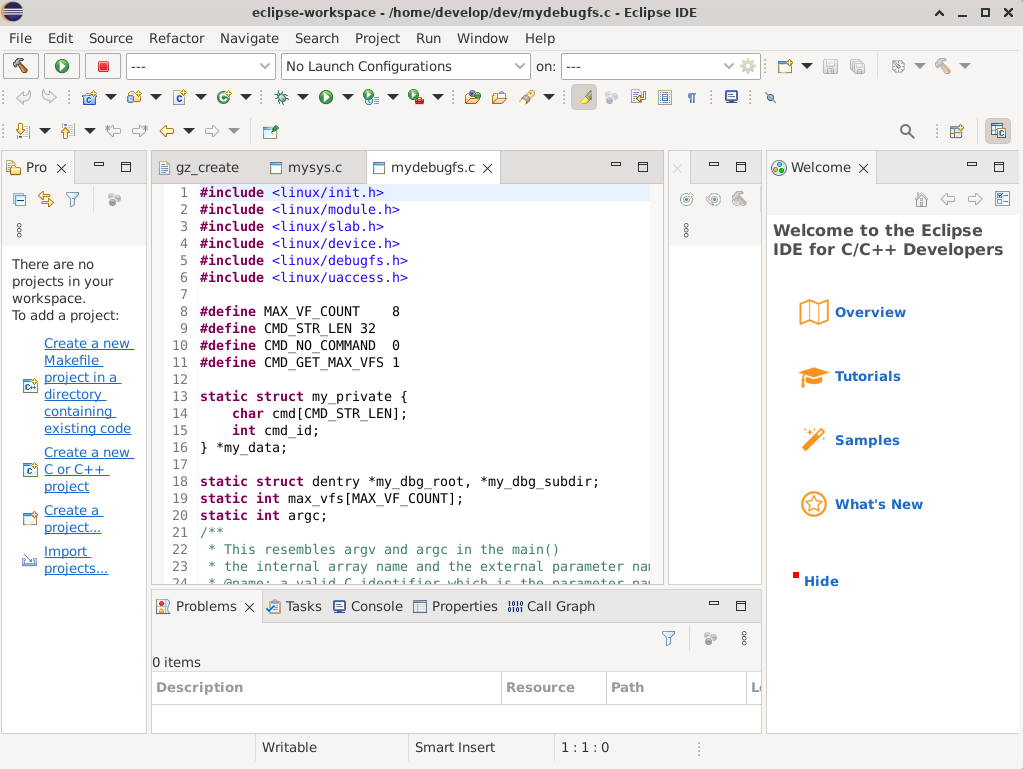
\includegraphics[width=\textwidth,height=0.6\textwidth]{images/eclipse.png}

    \subsection{vscode}
    這個 Microsoft 公司丟出來的 IDE ,後來隨著新畢業的小朋友帶進公司,很多人
    也都直接用這個,跟 eclipse 一樣,由於換組時,剛進去組裡的規矩規定環境操作
    方法,例如 source code 在哪,library 怎麼設定,參考文件都用 vscode ,所以
    我也被逼著用一下子,然後了解後,又用回熟悉的 vim, git 等命令。
    一樣可以\href{https://code.visualstudio.com/}{下載} Linux 版本。
    沒有權限的話,deb 可以用 ar 解開
    \begin{verbatim}
    ar vx code_1.86.2-1707854558_amd64.deb
    mkdir opt/vscode
    tar Jxvf data.tar.xz -C opt/vscode
    \end{verbatim}
    rpm 用 rpm2cpio 解開
    \begin{verbatim}
    mkdir -p opt/vscode; cd opt/vscode
    rpm2cpio code-1.86.2-1707854644.el8.x86_64.rpm | cpio -vid
    \end{verbatim}
    在裡面的 usr/share/code/bin 的執行檔執行。
    \\\\
    他裡面其實反而沒有 eclipse 的自創名詞,比較好懂,module 就 module, plugin
    就 plugin, extension 就 extension。
    \begin{itemize}
    \item workspace 這個是一個工作目錄,裡面有 project, source control 管理
      等資訊,而且這會跟 source control 有關,source control 通常會目錄下
      有好多支 branch ,則這樣會跟 workspace 打架,因此要特別注意使用。
    \item extension 等於是 module/plugin 我們好像一開始都會裝 ssh ,可是網路
      失敗時,他整個跳不出來,蠻爛的。另外副檔名的設定,也很誇張,內定居然
      file browser 不去讀沒支援的副檔名 extension。
    \item profile 某個大堆頭的整體設定
    \end{itemize}
    其實 microsoft 有個 packages.microsoft.com 網站,裡面的 repos 放了他們的
    Linux 軟體。

    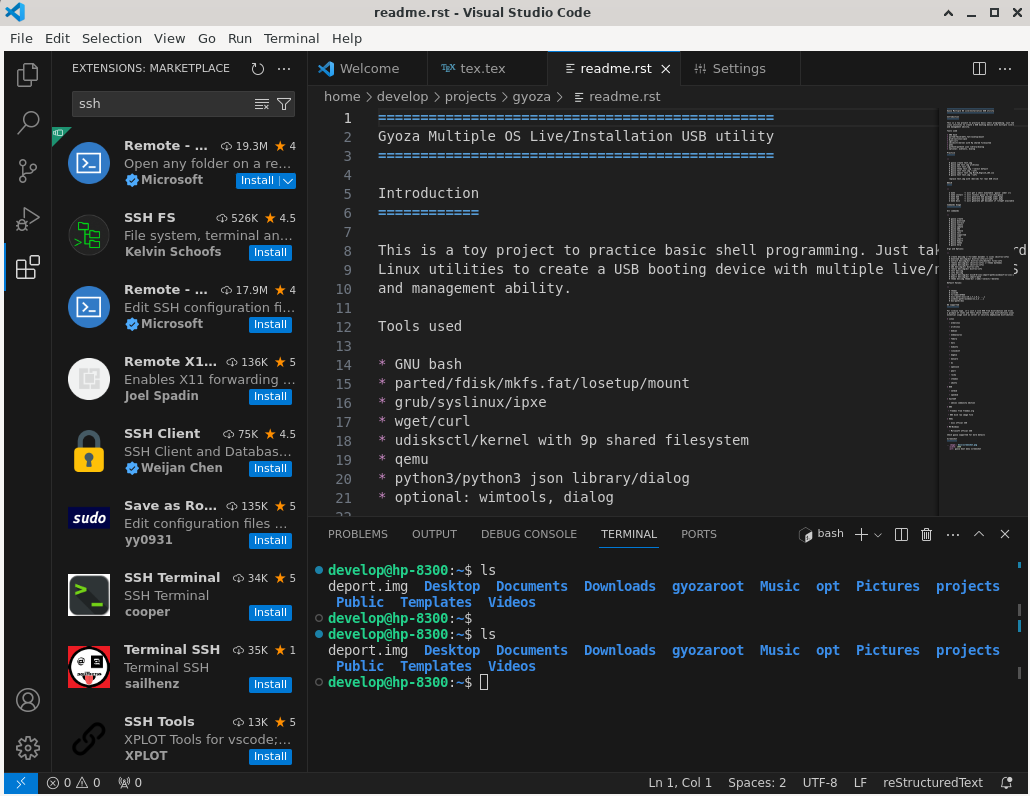
\includegraphics[width=\textwidth,height=0.6\textwidth]{images/vscode.png}

    \section{使用vim做一個IDE}
    我沒有很喜歡IDE,像 eclipse vscode,剛開始用,覺得不好用就是沒有習慣,
    真正要會用,也是真了解所有的步驟的含意,但真了解了,IDE 也不見得要有了。
    但菜鳥工程師除非是天才,不然一般人很難有習慣從心中完全想清楚規劃才 
    codeing, testing ,所以 IDE 對剛開始練習,嘗試有時還是有用。用熟練後,也
    蠻快速神奇的。做為一個IDE, 通常重要的就
    \begin{description}
      \item [file browser] \hfill \\
        可以像一般檔案夾那樣選擇檔案
      \item [include path的設定]\hfill \\
        PYTHONPATH,PERL5LIB, /usr/include, jar檔的引入
      \item [library path的設定] \hfill \\
        例如能設定PYTHONPATH, PERL5LIB, LD\_LIBRARY\_PATH,jar 檔引入,讓
        環境自動找到想用程式庫。
      \item [編譯] \hfill \\
        命令像make, java, mvn之類的呼叫,與出錯的除錯跳躍。
      \item [code completion] \hfill \\
        自動完成變數, API等的輸入。
      \item [syntax checking] \hfill \\
        語法的顏色與檢查
      \item [break point 與 run]
        能設定break point與執行程式並且一步步 trace
      \item [debug console] 
        能除錯及對於stdin/stdout/stderr的控制,通常也有 terminal 窗窗在大
        window 下。
    \end{description}
    除了可以使用.vimrc來初始vim外,.vim/plugin是個可以放特殊vim plugin的地方,
    作為一個IDE,推荐的plugin有
    \begin{itemize}
      \item \href{https://github.com/tpope/vim-pathogen}{pathogen}
      \item \href{https://github.com/scrooloose/nerdtree}{nerdtree}
      \item \href{https://github.com/ervandew/supertab}{supertab}
      \item \href{https://github.com/Valloric/YouCompleteMe}{YouCompleteMe}
      \item \href{https://github.com/scrooloose/syntastic}{Syntastic}
    \end{itemize}
    最簡單基本用法就是git下載後,把裏面的東西copy到.vim下就可以了。在vim官網中
    有一些\href{http://vim.wikia.com/wiki/Use\_Vim\_like\_an\_IDE}{介紹}

      \subsection{neovim}
      目前有一個新的 vim 替代品為 neovim,他的 IDE plugin 基本上更簡單安裝,
      \begin{itemize}
        \item \href{https://github.com/neovim/neovim/blob/master/INSTALL.md}{下載 neovim}
        \item 安裝 lazyvim plugin
        \begin{verbatim}
git clone https://github.com/LazyVim/starter \$HOME/.config/nvim
        \end{verbatim}
        \item 要花俏的外觀要裝
          \begin{itemize}
            \item \href{https://www.nerdfonts.com/}{nerd font} 這是 lazyvim
              會用到字型。選 JetBrain,在 linux 中放到 \$HOME/.fonts 並且
              mkfontscale
            \item \href{https://sw.kovidgoyal.net/kitty/}{kitty terminal},
              這是 optional 的 terminal,因為 gnome-termianl, xfce4-terminal
              都可以顯示漂亮的 nerd font。
              linux 中,export GLFW\_IM\_MODULE=ibus 然後啟動 kitty
          \end{itemize}
        \item 啟動 nvim
      \end{itemize}
      就有一個不錯的vim IDE。
      \begin{center}
      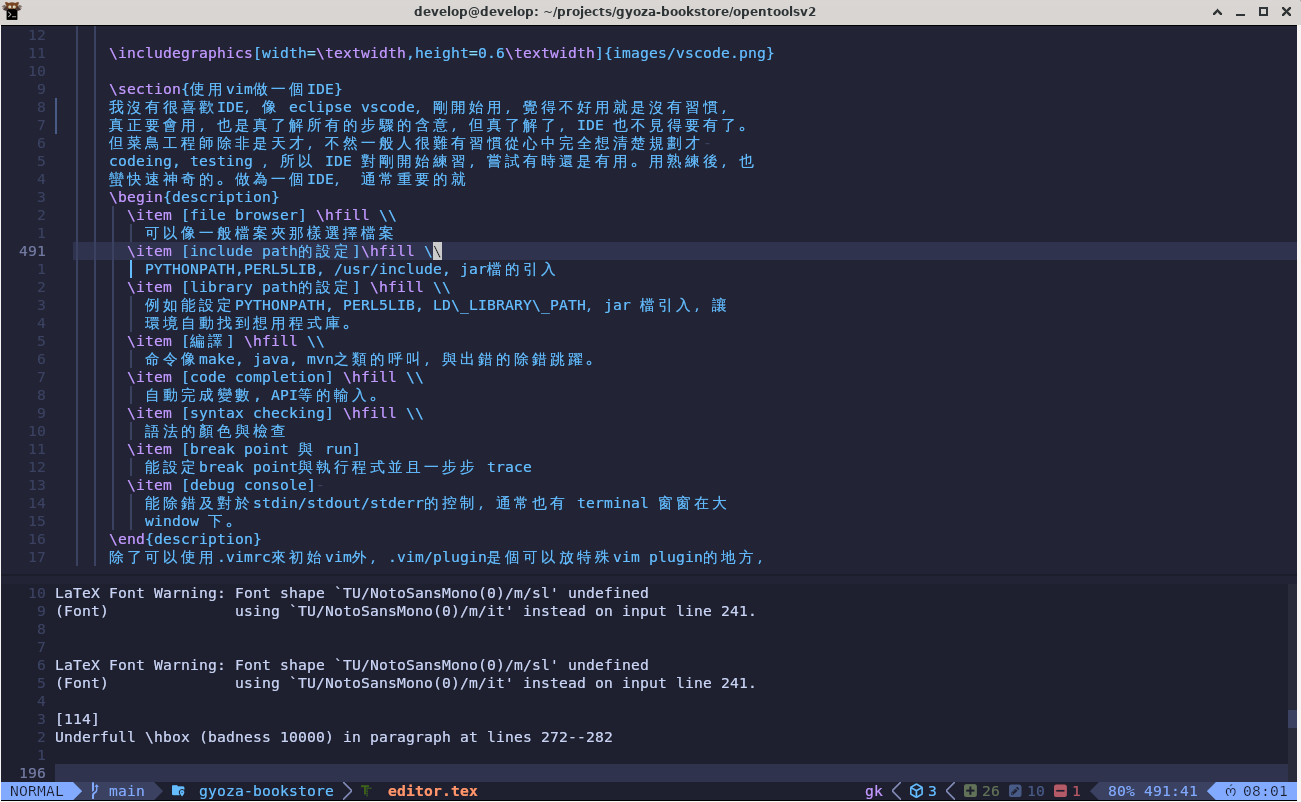
\includegraphics[width=\textwidth,height=0.6\textwidth]{images/nvim.png}
      \end{center}
      nvim 的設定主要是在 \$HOME/.config/nvim/init.lua,是個 lua script,然
      後主要安裝 lazyvim 這個簡易 plugin 就有自動補全的功能。如果要把原本
      .vimrc 的設定搬進來,在 init.lua 中使用 vim.cmd(),例如
      \begin{verbatim}
vim.cmd(set hidden)
      \end{verbatim}

    \section{其他輔助工具}
    其實shell本身就是非常強大的字串處理程式,加上sed/awk與其他工具,都能處理
    很複雜的問題了。但有些文字工具是對程式師特有的。
    \begin{itemize}
      \item grep -r pattern 搜尋子目錄下檔案裡面 pattern 的字串。解 bug 通常第
        一件事就是看錯誤訊息在哪裡。
      \item ctags/etags 建造變數,定義,函數等symbol的跳跳index。
      \item cscope 跟ctags很像,但他還能找特別的string,不光是特殊symbol。通常
        cscope/ctags是合併一起用。cscope -R -q 會產生
      \begin{itemize}
        \item cscope.out      Symbol交叉參考(cross-reference)檔
        \item cscope.in.out   反向索引檔用來做快速Symbol
        \item cscope.po.out   反向索引檔
      \end{itemize}
      要結束請按ctrl-D
      \item indent 根據自訂條件的indentation再處理。
      \item diff 與 vimdiff 比對兩個檔案的差異。
        \begin{itemize}
          \item diff -puN : print the c function and 3 lines of unified context
          \item diff -ruN : 產生一個patch檔,file.diff, patch -p1 \verb=<= file.diff;
          \item diff -yN : two column
        \end{itemize}
        vimdiff 可以直接在兩個檔案編輯,通常在解決 merge conflict 的時候很有用。
      \item patch 兩個檔案差異的對前一版的修訂。這比較重要的就是使用p0或p1選項
        ,例如source在myproj-1.0目錄,則使用diff產生的patch檔,站在myproj-1.0
        外面就是 patch -p1 \verb=<= mypatch, cd myproj-1.0後就是 patch -p0 
        \verb=<= mypatch,現在也很多用 git diff, git apply 來作業。
      \item tmux 與 screen 是在 terminal 上畫出多個窗窗工作的軟體,兩派也激戰
        很久,screen 有個好處是他同時可作 rs232 console port 的 terminal ,
        但 tmux 有很多新進處理比 screen 好。他們的主要用法是先給一個前置命令
        按鍵表示後續按鍵是軟體命令,差別就是前置按鍵
        \\\\
        tmux, 術語中, pane 表示真實切割畫面,window 表示虛擬 terminal+shell
        \begin{itemize}
          \item 開水平pane Ctrl-b " (split)
          \item 開垂直pane Ctrl-b \%
          \item 開虛擬window Ctrl-b c  (neww)
          \item 跳到下一個window Ctrl-b n (next)
          \item 跳到上一個window Ctrl-b p (prev)
          \item 跳到下一個pane Ctrl-b 上下左右
          \item 關閉pane Ctrl-b x (kill-pane)
          \item 進到命令列 Ctrl-b :  (這跟 vi 是很像,冒號後跟命令)
          \item 調整pane 大小 Ctrl-b Ctrl-上下左右
        \end{itemize}
        screen,用術語 region 表示真的切割畫面, window 表示虛擬 terminal+shell
        \begin{itemize}
          \item 開水平region Ctrl-a S  (split)
          \item 開垂直region Ctrl-a |  (split -v)
          \item 開虛擬window Ctrl-a c  (create)
          \item 跳到下一個window Ctrl-a n (next)
          \item 跳到上一個window Ctrl-a p (prev)
          \item 跳到下一個region Ctrl-a tab (focus)
          \item 關閉region Ctrl-a X (remove)
          \item 進到命令列 Ctrl-a : (這跟 vi 很像,冒號後跟命令)
          \item 列出window Ctrl-a " (windowlist -b)
          \item screen /dev/ttyS1 變成 serial port 1 的 console
        \end{itemize}
      \item a2ps 古老以前code review,我們是印出來的,現在都是線上code
        review。這在/etc/a2ps.cfg下可以全域設定。通常duplex印雙面,調整
        紙張大小letter-lj之類的。
    \end{itemize}
    \section{結語}
    不管是哪種editor,最重要的就是整組人馬是用同一種coding style, 用同一種
    indentation, 同一種換行,同一種習慣,這在將來code的維護,branch的merge
    ,開發,測試,除錯的循環中會影響效率非常的大。每個好的editor都是可以調整
    的,所以一定要把規矩講清楚,大家來遵守。至於要用 vim, emacs, neovim, 
    atom, eclipse, vscode, sublime ...其實都無所謂。
